\documentclass[11pt]{article}
\usepackage{graphicx}
\usepackage{amsmath}
\usepackage{float}
\usepackage{indentfirst}
\usepackage{array, amsmath}
\usepackage{stackengine}

    \title{\textbf{Midterm Exam}}
    \author{Ameya Konkar  UID:118191058}
    \date{}
    
    \addtolength{\topmargin}{-3cm}
    \addtolength{\textheight}{3cm}
\begin{document}

\maketitle
\thispagestyle{empty}

\section{Question 1}
Following are the steps to equilize the histogram of an image using \textbf{Normal} and \textbf{Contrast Limited Advanced Histogram Equilazation}.

\begin{description}
\addtolength{\itemindent}{0.80cm}
\itemsep0em 
\item[a)] \textbf{Histogram Equilization}
\item[1.] Counted total number of pixels of every intensity from (0-255) present in the grayscaled images. 
\item[2.] Stored the pixels present in particular groups.
\item[3.] Calculated \textbf{cdf} of every intensity from (0-255).
\item[4.] Changed the intensity of the stored pixels for every group from (0-255) with \textbf{cdf[i]*i}.
\newline
\item[b)] \textbf{Contrast Limited Advanced Histogram Equilazation}
\item[1.] Divided the image in 8x8 parts.
\item[2.] For every part, counted total number of pixels of every intensity from (0-255) present in the grayscaled images. 
\item[3.] Stored the pixels present in particular groups.
\item[4.] Calculated \textbf{pdf} of every intensity from (0-255).
\item[5.] Clipped every bucket of each intensity with a predifined value. Distributed the extra values collected equally in every intensity buckets.
\item[5.] Calculated new \textbf{cdf} and changed the intensity of the stored pixels for every group from (0-255) with \textbf{cdf[i]*i}.

Out of the two approaches \textbf{Contrast Limited Advanced Histogram Equilazation} is \textbf{better}. It performs histogram equilization on seperate blocks hence avoiding oversaturation of certain parts of the image. 

\begin{figure}[H]
  \centering
	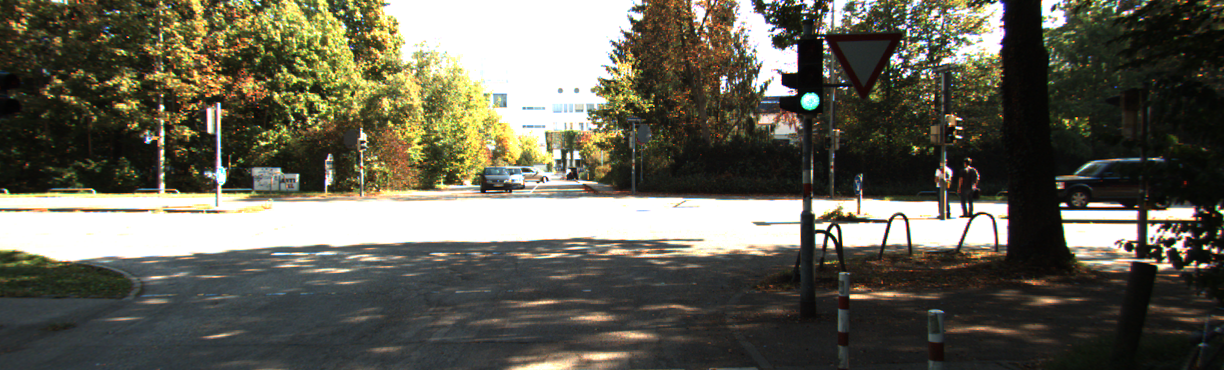
\includegraphics[width=1\textwidth]{orig_img}
	\caption{Original Image.} 
\end{figure}

\begin{figure}[H]
  \centering
	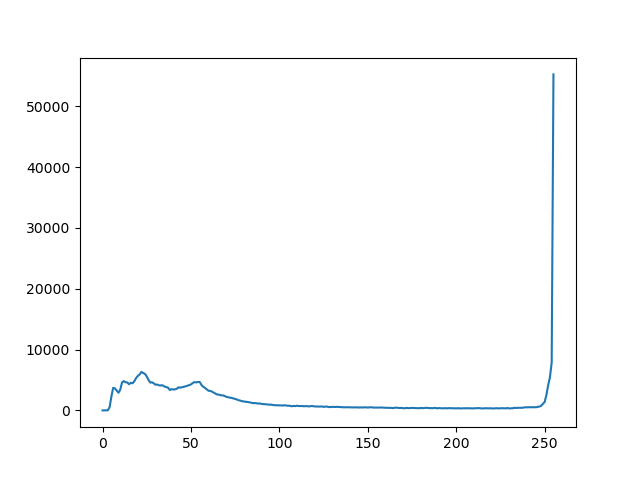
\includegraphics[height=0.7\textwidth]{Q1_a_img_hist}
	\caption{Histogram of original grayscaled image.} 
\end{figure}

\begin{figure}[H]
  \centering
	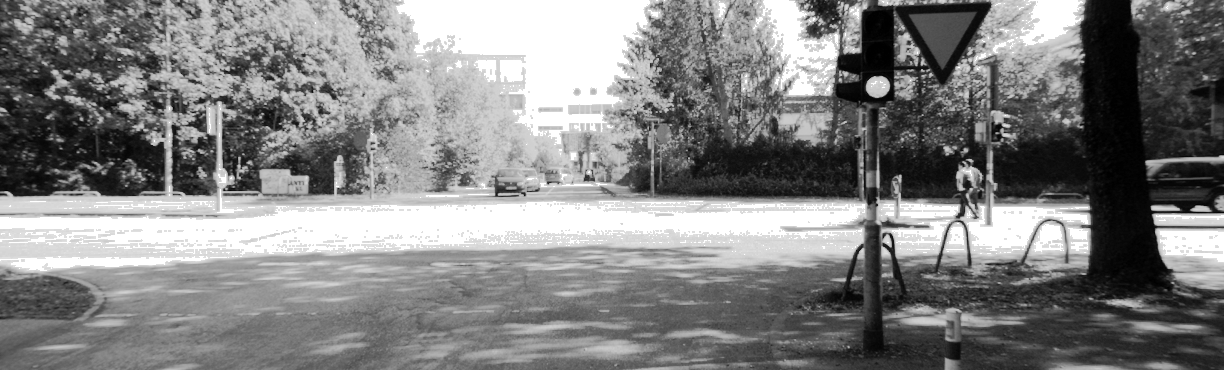
\includegraphics[width=1\textwidth]{Hist}
	\caption{Normal Histogram Equilization.} 
\end{figure}


\begin{figure}[H]
  \centering
	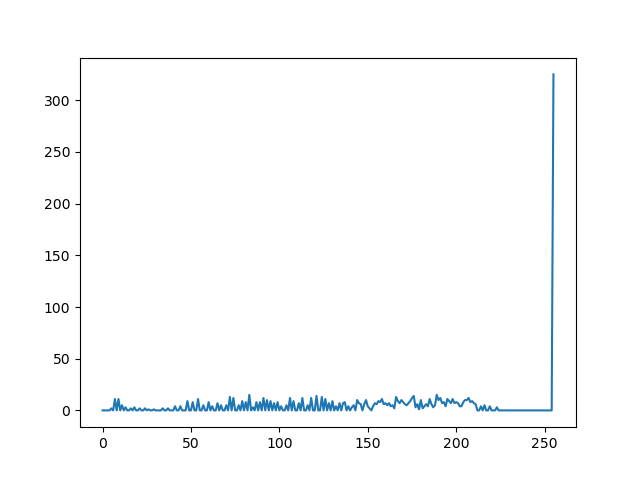
\includegraphics[width=1\textwidth]{Q1_a_nhe}
	\caption{Normal Histogram Equilization.} 
\end{figure}

\begin{figure}[H]
  \centering
	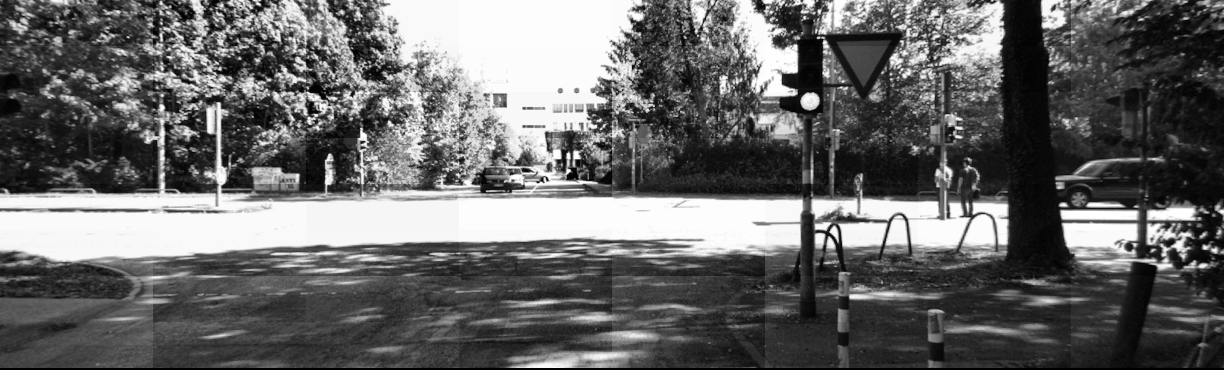
\includegraphics[width=1\textwidth]{CLAHE}
	\caption{Contrast Limited Advanced Histogram Equilazation.} 
\end{figure}

\begin{figure}[H]
  \centering
	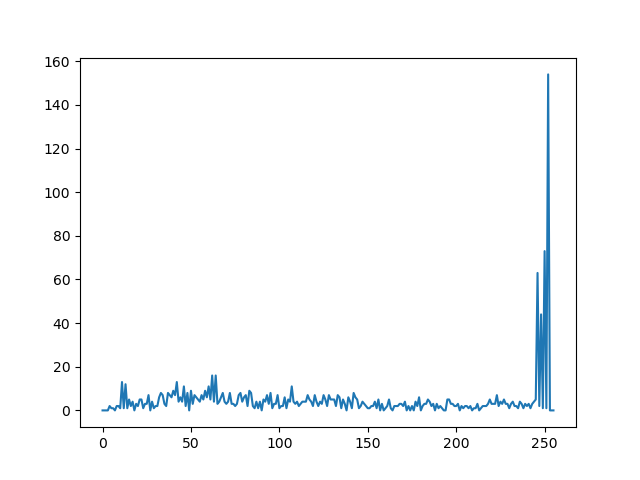
\includegraphics[width=1\textwidth]{Q1_b_clahe}
	\caption{CLAHE histogram} 
\end{figure}


\end{description}

\section{Question 2}
Following are the steps to detect lanes in given images.
\begin{description}
\addtolength{\itemindent}{0.80cm}
\itemsep0em 
\item[1.] Coverted the copies of the given images in grayscale.
\item[2.] Considered a trapezium part of the image containing two lanes.
\begin{figure}[H]
  \centering
	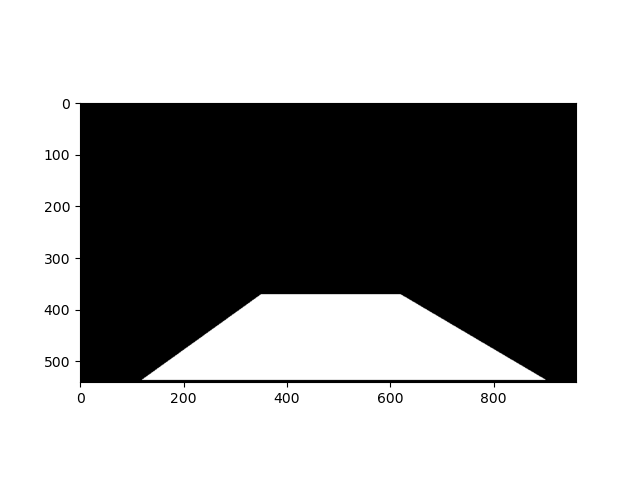
\includegraphics[height=0.7\textwidth]{Q2_stencil}
	\caption{Stencil to extract lane image.} 
\end{figure}
\begin{figure}[H]
  \centering
	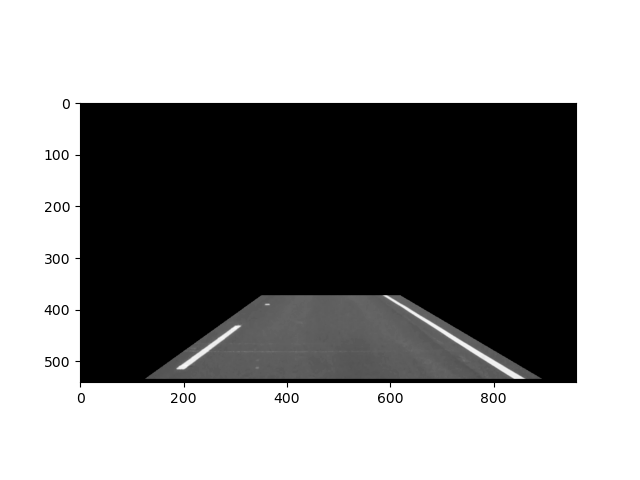
\includegraphics[height=0.7\textwidth]{Q2_gray}
	\caption{Extracted Lane image.} 
\end{figure}
\item[3.] Detected lanes using Hough lines.
\item[4.] Rejected similar lineson the same lane.
\item[5.] Differentiated the lanes by coloring them with green and red.

\begin{figure}[H]
  \centering
	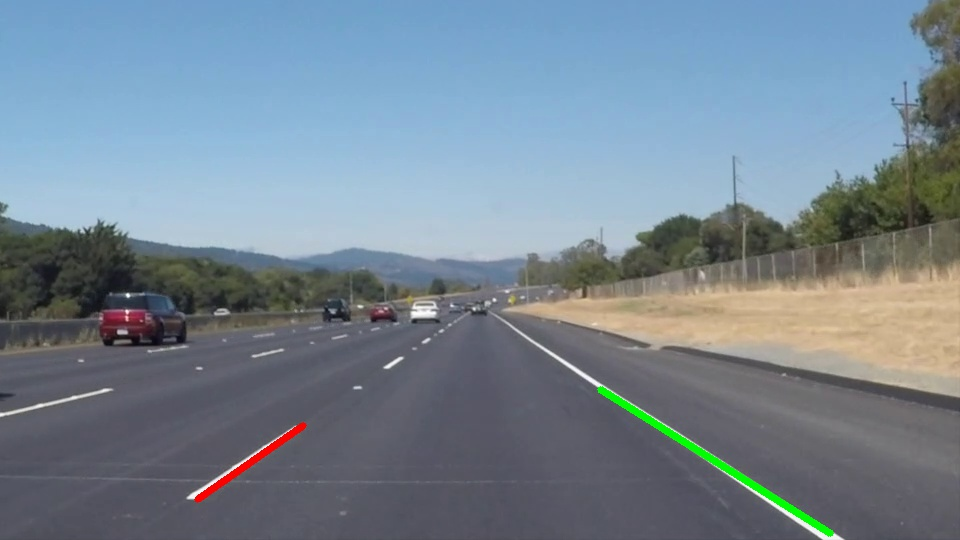
\includegraphics[height=0.4\textwidth]{Q2_main}
	\caption{Lane Detection.} 
\end{figure}

\end{description}

\section{Question 3}
Following are the steps to find the radius of curvature of the detected lanes.
\begin{description}
\addtolength{\itemindent}{0.80cm}
\itemsep0em 
\item[1.] Converted the copies of the given images in grayscale.
\item[2.] Considered a trapezium part of the image containing two lanes.
\item[3.] Warped the part to get a frame containing the lanes
\begin{figure}[H]
  \centering
	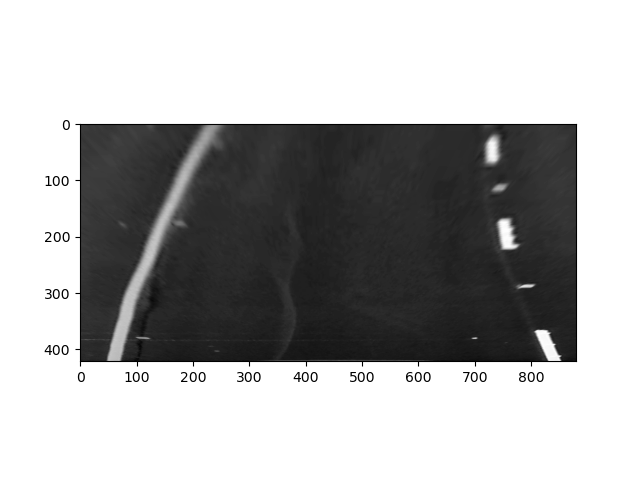
\includegraphics[height=0.7\textwidth]{gray}
	\caption{Warped Image} 
\end{figure}
\item[4.] The warped image was then thresholded.
\begin{figure}[H]
  \centering
	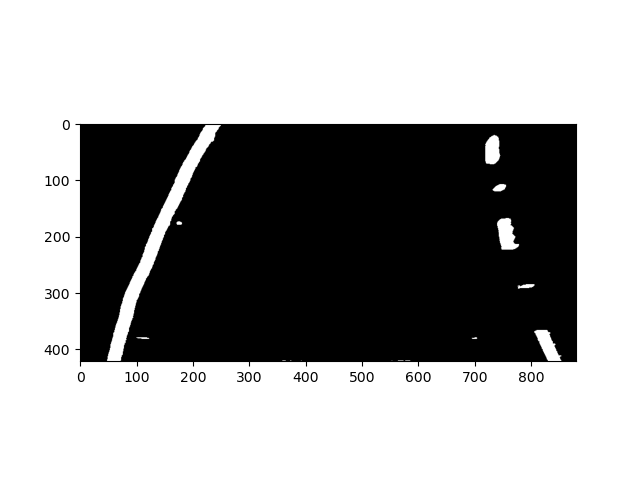
\includegraphics[height=0.7\textwidth]{thresh}
	\caption{Thresholded Warped Image} 
\end{figure}
\item[5.] Implemented the sliding window approach to detect multiple points on the lanes which will then be used to detect the curvature of the lanes.

\begin{figure}[H]
  \centering
	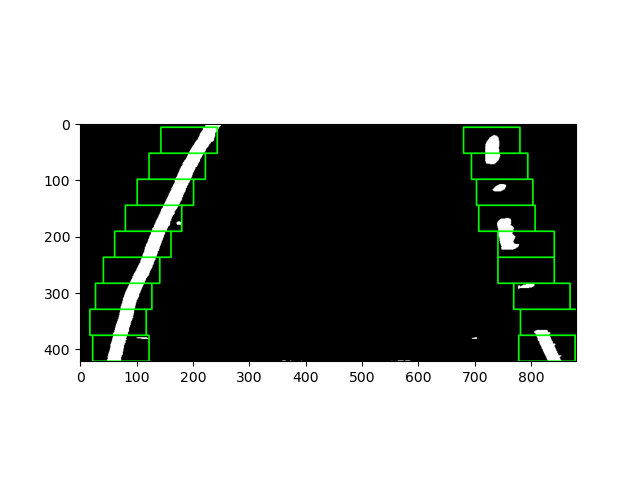
\includegraphics[height=0.7\textwidth]{thresh1}
	\caption{Lane Detection.} 
\end{figure}

\item[6.] Based on the curvature of the lane, indicated the vehicle to turn right, left or moving straight is found.
\begin{figure}[H]
  \centering
	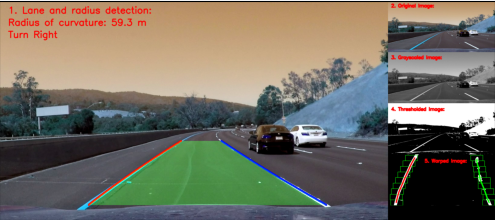
\includegraphics[height=0.5\textwidth]{main(1)}
	\caption{Final Frame} 
\end{figure}

Following is the brief explaination of \textbf{Sliding Window approach} uesd in lane detection.
\addtolength{\itemindent}{0.80cm}
\item[a)] \textbf{Sliding Window Approach}

\item[i.] Found histogram of white pixels along the x-axis in the warped and thresholded image.
\item[ii.] Divided the array having the number of white pixels for every column in x-axis in two parts.
\item[iii.] Found x position in both parts of the array.
\item[iv.] Considered two rectangular block around the two x coordinates found.
\item[v.] The block size is considered as 1/9*height of the image height.
\item[vi.] The first blocks are considered at the bottom of the image. Thus shifting the blocks upwards and considered 9 blocks per side per image frame.
\item[vii.] In every block, found the mean of the x-coordinates of the white coordinates present as the new white coordinate present.  
\item[viii.] The steps from v to viii is repeated for every frame.   

\item[b)] \textbf{Understanding of Homography}
The homography is performed by calculating the Homography matrix.
The homography matrix can be computed as the eigen vector corresponding to the least eigen value
The A matrix consists of atleast 4 points from the image space and corresponding world space.
In the given frames, 4 points corresponding to the image are selected and homography transformation is performed based on those 4 points.

\item[c)] \textbf{Understanding of Hough lines}
The hough lines are found by projecting the points in r, theta space. For each point, a wave appears in that space. Intersection of the waves of multiple points indicate that the points lie on the same line.

\item[d)] \textbf{How likely will the pipeline generalize}
The pipeline is generalized to the scenarios faced in the given videos. If any other issue occurs, then it may face issues.

\end{description}

\end{document}

